%\setcounter{chapter}{29}
\chapter{Representation Learning}\label{chapter:representation_learning}

\section{Introduction}
In this book we have seen many ways to represent visual signals: in the spatial domain versus frequency domain, with pyramids and filter responses, and more. We have seen that the choice of representation is critical: each type of representation makes some operations easy and others hard. We also saw that deep neural networks can be thought of as transforming the data, layer by layer, from one representation into another and another.%, and, as we will soon see, those representations are transferable. 
If representations are so important, why not set our objective to be ``come up with the best representation possible.'' In this chapter, we will try to do exactly that.

This chapter is primarily an investigation of \textit{objectives}. We will identify different objective functions that capture properties of what it means to be a good representation. Then we will train deep nets to optimize these objectives, and investigate the resulting learned representations.

\section{Problem Setting}
Before diving in, let us present the basic problem statement and the notation we will be using throughout this chapter.

The goal of representation learning is to learn to map from datapoints, $\mathbf{x} \in \mathcal{X}$, to abstract representations, $\mathbf{z} \in \mathcal{Z}$, as schematized in \fig{\ref{fig:representation_learning:rep_learning_schematic}}:

\begin{figure}[h!]
    \centerline{
        \includegraphics[width=.52\linewidth]{figures/representation_learning/rep_learning_schematic.pdf}
    }
    %\vspace{-1.0em}
    \caption{The goal in this chapter is to learn to map from datapoints to abstract representations, which are typically simpler and more useful than the raw data.}\label{fig:representation_learning:rep_learning_schematic}
\end{figure}

We call this mapping an {\bf encoding} and learn an \index{Encoder}{\bf encoder} function $f: \mathcal{X} \rightarrow \mathcal{Z}$. Typically both $\mathbf{x}$ and $\mathbf{z}$ are high-dimensional vectors, and $\mathbf{z}$ is called a \index{Vector embedding}{\bf vector embedding} of $\mathbf{x}$. The mapping $f$ is trained so that $\mathbf{z}$ has certain desirable properties: common desiderata include that $\mathbf{z}$ be lower dimensional than $\mathbf{x}$; that the distribution of $\mathbf{z}$ values, that is, $p(\mathbf{z})$, has a simple structure (such as being the unit normal distribution); and that the dimensions of $\mathbf{z}$ be independent factors of variation, that is, the representation should be \index{Disentangled representation}\textbf{disentangled}~\cite{bengio2013representation}. In this way $\mathcal{Z}$ is a simpler, more abstracted, or better organized representational space than $\mathcal{X}$, as reflected in the shapes in \fig{\ref{fig:representation_learning:rep_learning_schematic}}.

\section{What Makes for a Good Representation?}

A good representation is one that makes subsequent problem solving easier. Below we discuss several desiderata of a good representation.

\subsection{Compression}
A good representation is one that is parsimonious and captures just the essential characteristics of the data necessary for tasks of human interest. There are at least three senses in which compressed representations are desirable.
\begin{enumerate}
    \item Compressed representations require less memory to store.
    \item Compression is a way to achieve invariance to nuisance factors. Depending on what the representation will be used for, nuisances might include camera noise, lighting conditions, and viewing angle. If we can factor out those nuisances and discard them from our representation, then the representation will be more useful for tasks like object recognition where camera and lighting may change without affecting the semantics of the observed object.
    \item Compression is an embodiment of \textit{Occam's razor}: among competing hypotheses that all explain the data equally well, the simplest is most likely to be true. As we will see below, and in the next chapter, many representation learning algorithms seek simple representations from which you can regenerate the raw data (e.g., autoencoders). Such representations explain the data in the formal sense that they assign high likelihood to the data. This is the same sense to which the idea of Bayesian Occam's razor applies (\sect{\ref{sec:problem_of_generalization:star_problem_revisited}}); see \cite{mackay2003information} for a mathematical treatment of this idea. Therefore, we can state Occam's razor for representation learning: among two representations that fit the data equally well, give preference to the more compressed.\marginnote{This version of Occam's razor is also known as the \index{Minimum description length principle}\textbf{minimum description length principle}~\cite{grunwald2007minimum}}[-0.8cm]
          %simple representations are more likely to be ``true" (we will unpack this idea below).
\end{enumerate}

Many representation learning algorithms capture these goals by penalizing or constraining the complexity of the learned representation. Such a penalty must be paired with some other objective or else it will lead to a degenerate solution: just make the representation contain nothing at all. Usually we try to compress the signal in certain ways while preserving other aspects of the information it carries. \textit{Autoencoders} and \textit{contrastive learning}, which we will describe subsequently, are two representation learning algorithms based on the idea of compression.

%One idea is to just remove all the redundant bits of information. This idea is captured by autoencoders. Another idea is to remove all bits that are not shared between different ways of viewing the world. That idea is called contrastive learning.

\subsection{Prediction}
The whole purpose of having a visual system is to be able to take actions that achieve desirable future outcomes. Predicting the future is therefore very important, and we often want representations that act as a good substrate for prediction. %An extreme version of this idea is to simply represent a signal with prediction of its future state, and idea called {\bf predictive coding}. For example, as we listen to spoken words our representation of the word ``mashed" might be a prediction of the words that may follow, e.g., ``potatoes". It's a weird concept -- you represent one word with another -- but it works quite well, especially when our representation is not just a single prediction but a distribution over possible next words. Then the word ``mashed" might get represented as a probability mass distribution over $N$ possible future words, with high mass on ``potatoes", ``yams", ``cauliflower", etc.

The idea of prediction can be generalized to involve more than just predicting the \textit{future}. Instead we may want to predict the past (i.e., given when I'm seeing today, what happened yesterday?), or we may want to predict gaps in our measurements, a problem known as {\bf imputation}. Filling in missing pixels in a corrupted image is an example of imputation, as is superresolving a movie to play at a higher framerate. We may even want to perform more abstract kinds of predictions, like predicting what some other agent is thinking about (a problem called theory of mind). In general, prediction can refer to the inference of any arbitrary property of the world given observed data. Facilitating the prediction of important world properties—the future, the past, mental states, cause and effect, and so on—is perhaps the defining property of a good representation.

Most representation learning algorithms in vision are about learning compressed encodings of the world that are also predictive of the future (and therefore a good substrate for decision making). Beyond just compression and prediction, some works have explored other goals, including that a representation be disentangled~\cite{bengio2013representation}, interpretable~\cite{koh2020concept}, and actionable~\cite{soatto2013actionable} (you can use it as an effective substrate for control). All these goals—compression, prediction, interpretability, and so on—are not in contrast to each other but rather overlap; for example, more compressed representations may be simpler and hence easier for a human to interpret.

%\paragraph{Imputation}
%Imputation is a generalization of the idea of prediction. Rather than just predicting the \textit{future}, imputation is the inference of \textit{any} missing data. Imagine you have some data tensor, e.g., a movie that extends in both space and time. The movie is only sampled a particular resolution, and a particular temporal rate. Imputation is the problem of inferring all the gaps -- what would the movie look like at a higher sampling rate? Or perhaps the movie is corrupted and some pixels are missing. Inferring those pixel values is also an imputation problem.

%\paragraph{Empowerment} We also might want representations that facilitate control.


\subsection{Types of Representation Learners}

Representation learning algorithms are mostly differentiated by the objective function they optimize, as well as the constraints on their hypothesis space. We explore a variety of common objectives in the following sections, and summarize how these relate to the core principles of compression and prediction in \tab{\ref{tab:representation_learning:types_of_representation_learners}}.

\begin{table}[]
    \caption{One way to categorize different representation learning methods.} % Hack to get the caption of the table in the margin.
    %\marginnote{{\bf Table \ref{tab:representation_learning:types_of_representation_learners}}: One way to categorize different representation learning methods.} % Hack to get the caption of the table in the margin.
    %\faketablecaption{} % this updates the counter without plotting a caption.
    \begin{center}
        \begin{tabular}{ccc}
            \toprule
            \textbf{Learning} & \textbf{Learning}  &                                                   \\
            \textbf{Method}   & \textbf{Principle} & \textbf{Short Summary}                            \\
            \midrule
            Autoencoding      & Compression        & Remove redundant information                      \\
            Contrastive       & Compression        & Achieve invariance to viewing transformations     \\
            Clustering        & Compression        & Quantize continuous data into discrete categories \\
            Future prediction & Prediction         & Predict the future                                \\
            Imputation        & Prediction         & Predict missing data                              \\
            Pretext tasks     & Prediction         & Predict abstract properties of your data          \\
            \bottomrule
        \end{tabular}
    \end{center}
    %\caption{One way to categorize different representation learning methods.}
    \label{tab:representation_learning:types_of_representation_learners}
\end{table}

%, including \textit{autoencoding}, \textit{predictive coding}, \textit{pretext tasks}, \textit{imputation}, \textit{clustering}, and \textit{contrastive learning}.

\section{Autoencoders}\label{sec:representation_learning:autoencoders}

\index{Autoencoders}{\bf Autoencoders} are one of the oldest and most common kinds of representation learners~\cite{rumelhart1985learning, ballard1987modular}. An autoencoder is a function that maps data back to itself (hence the ``auto''), but via a low-dimensional representational \textbf{bottleneck}, as shown in \fig{\ref{fig:representation_learning:autoencoder_diagram}}:
\begin{figure}[h!]
    \centerline{
        \includegraphics[width=1.0\linewidth]{figures/representation_learning/autoencoder_diagram.pdf}
    }
    \caption{{\small (left) An autoencoder maps from points in data space, to points in representation space, and back. (right) An example of running an autoencoder on an input image of a bird.}}\label{fig:representation_learning:autoencoder_diagram}
\end{figure}

On the right of this figure is an example of an autoencoder applied to an image. At first glance this might not seem very useful: the output is the same as the input! The key trick is to impose constraints on the intermediate representation $\mathbf{z}$, so that it becomes useful. The most common constraint is compression: $\mathbf{z}$ is a low-dimensional, compressed representation of $\mathbf{x}$.

To be precise, an autoencoder $F$ consists of two parts, an \index{Encoder}\textbf{encoder} $f$ and a \index{Decoder}\textbf{decoder} $g$, with $F = g \circ f$. The encoder, $f: \mathbb{R}^N \rightarrow \mathbb{R}^M$, maps high-dimensional data $\mathbf{x} \in \mathbb{R}^N$ to a vector embedding $\mathbf{z} \in \mathbb{R}^M$. Typically, the key property is that $M < N$, that is, we have performed \index{Dimensionality reduction}{\bf dimensionality reduction} (although autoencoders can also be constructed without this property, in which case they are not doing dimensionality reduction but instead may place other explicit or implicit constraints on $\mathbf{z}$). The decoder, $g: \mathbb{R}^M \rightarrow \mathbb{R}^N$ performs the inverse mapping to $f$, and ideally $g$ is exactly the inverse function $f^{-1}$. Because it may be impossible to perfectly invert $f$, we use a loss function to penalize how far we are from perfect inversion, and a typical choice is the squared error \index{Reconstruction loss}\textbf{reconstruction loss}, $\mathcal{L}_{\texttt{recon}}(\hat{\mathbf{x}}, \mathbf{x}) = \norm{\hat{\mathbf{x}} - \mathbf{x}}_2^2$. Then the learning problem is:
\begin{equation}
    f^*,g^* = \argmin_{f,g} \mathbb{E}_{\mathbf{x}} \norm{g(f(\mathbf{x})) - \mathbf{x}}_2^2 \label{eqn:representation_learning:autoencoder_learning_problem}
\end{equation}
The idea is to find a lower dimensional representation of the data from which we are able to reconstruct the data. An autoencoder is fine with throwing away any redundant features of the raw data but is not happy with actually losing information. The particular loss function determines what kind of information is preferred when the bottleneck cannot support preserving \textit{all} the information and a hard choice has to be made. The $L_2$ loss decomposes as $\norm{g(f(\mathbf{x})) - \mathbf{x}}_2^2 = \sqrt{\sum_i (g(f(\mathbf{x}))_i - x_i)^2}$, that is, a sum over individual pixel errors. This means that it only cares about matching each individual pixel intensity $g(f(\mathbf{x}))_i$ to the ground truth $x_i$ and does not directly penalize patch-level statistics of $\mathbf{x}$ (i.e., statistics $\phi(\mathbf{x})$ that do not factorize as a sum $\sum_i \psi_i(x_i)$ over per-pixel functions $\psi_i$ for any possible set of functions $\{\psi_i\}$). Autoencoders can also be constructed using loss functions that penalize higher-order statistics of $\mathbf{x}$, and this allows, for example, penalizing errors in the reconstruction of edges, textures, and other perceptual structures beyond just pixels~\cite{snell2017learning}.%, and this requires using a loss function that does not factorize into a product over individual pixel matching.
%The $L_2$ loss says preserve as much variance as possible in the reconstructed data distribution. This is because we can write the objective as $X\hat{X}$.... %A special case of an autoencoder with this objective is PCA -- PCA is simply an $L_2$ autoencoder for which $f$ and $g$ are both linear functions.

The learning diagram for the basic $L_2$ autoencoder looks like this:
\begin{center}
    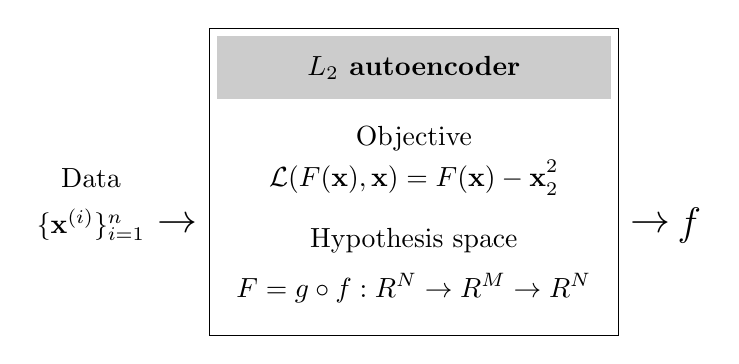
\begin{tikzpicture}
        \draw (0,0) rectangle (5.2,3.9); % outer box
        \fill[black!20] (0.1,3.0) rectangle (5.1,3.8); % gray box
        \node[] at (2.6,3.4) {{\bf $L_2$ autoencoder}};
        \node[] at (2.6,2.5) {Objective}; \node[] at (2.6,2.0) {$\mathcal{L}(F(\mathbf{x}), \mathbf{x}) = \norm{F(\mathbf{x}) - \mathbf{x}}_2^2$};
            \node[] at (2.6,1.2) {Hypothesis space}; \node[] at (2.6,0.6) {$F = g \circ f: \mathbb{R}^N \rightarrow \mathbb{R}^M \rightarrow \mathbb{R}^N$};
            \node[] at (-1.5,2.0) {Data};
            \node[] at (-1.5,1.4) {$\{\mathbf{x}^{(i)}\}_{i=1}^n$};
        \node[] at (-0.4,1.4) {{\Large  $ \rightarrow$}};
        \node[] at (6.1,1.4) {{\Large $f$}};
        \node[] at (5.6,1.4) {{\Large  $ \rightarrow$}};
    \end{tikzpicture}
\end{center}
The optimizer is arbitrary but a typical choice would be gradient descent. The functional form of $f$ and $g$ are typically deep neural nets. The output is a learned data encoder $f$. We also get a learned decoder $g$ as a byproduct, which has its own uses, but, for the purpose of representation learning, is usually discarded and only used as scaffolding for training what we really care about, namely $f$.

Closely related to autoencoders are other dimensionality reduction algorithms like \index{Principle components analysis}\textbf{principle components ananlysis} (\textbf{PCA}). In fact, an $L_2$ autoencoder, for which both $f$ and $g$ are linear functions, learns an $M$-dimensional embedding that spans the same subspace as a PCA projection to $M$-dimensions~\cite{bourlard1988auto}.

\marginnote{Autoencoders may not seem like much at first glance, but they actually appear all over the place, and many methods in this book can be considered to be special kinds of autoencoders, if you squint. Two examples: the steerable pyramid from \chap{\ref{chapter:image_pyramids}} is an autoencoder, and the CycleGAN algorithm from \chap{\ref{chapter:generative_models}} is also an autoencoder. See if you can find more examples.}[0cm]

%[PCA-like example of disentangled latent space arrived at by an autoencoder?]

%\begin{tcolorbox}[colback=experiment_box_color]
\subsection{Experiment: Do Autoencoders Learn Useful Representations?}
It is clear from the above that autoencoders will learn a \textit{compressed} representation of the data, but do they learn a \textit{useful} representation? Of course the answer to this question depends on what we will use the representation for. Let's explore how autoencoders work on a simple data domain, consisting just of colored circles, triangles, and squares. The data consists of 64,000 images, samples of which are shown in \fig{\ref{fig:representation_learning:shapes_dataset_random_samples}}.
\begin{figure}[h!]
    \centerline{
        \includegraphics[width=0.275\linewidth]{figures/representation_learning/shapes_dataset_random_samples.pdf}
    }
    \caption{A sample from the toy dataset we will work with in this chapter.}
    \vspace{-1.0em}
    \label{fig:representation_learning:shapes_dataset_random_samples}
\end{figure}

Each shape has a randomized size, position, and rotation. Each shape's color is sampled from one of eight color classes (orange, green, purple, etc.) plus a small random perturbation.

For the autoencoder architecture we use a convolutional encoder and decoder, each with six convolutional layers interspersed with relu nonlinearities and a 128-dimensional bottleneck (i.e., $M=128$). We train this autoencoder for 20,000 steps of stochastic gradient descent, using the Adam optimizer~\cite{kingma2014adam} with a batch size of 128.

After training, does this autoencoder obtain a good representation of the data? To answer this question, we need ways of evaluating the quality of a representation. There are many ways and indeed how to evaluate representations is an open area of research. But here we will stick with a very simple approach: see if the nearest neighbors, in representational space, are meaningful.

We can test this in two ways: (1) for a given query, visualize the images in the dataset whose embeddings are nearest neighbors to the query's embedding, and (2) measure the accuracy of a one-nearest-neighbor classifier in embedding space. Below, in \fig{\ref{fig:representation_learning:AE_results_shapes_dataset}}, we show both these analyses.
\begin{figure}[h!]
    \centerline{
        (a) \includegraphics[width=0.38\linewidth]{figures/representation_learning/AE_NN_viz.pdf}
        (b) \includegraphics[width=0.40\linewidth]{figures/representation_learning/AE_NN_probe.pdf}
    }
    \caption{(a) Nearest neighbors, in autoencoder embedding space, to a set of query images. (b) Classification accurracy of a one-nearest-neighbor classifier of color and shape using the embeddings at each layer of the autoencoder's encoder.}
    \label{fig:representation_learning:AE_results_shapes_dataset}
\end{figure}
%\end{tcolorbox}

Recall that every layer of a neural net can be considered as an embedding (representation) of the data. On the left we show the nearest neighbors to a set of query images, using the layer 6 embeddings of the data as the feature space in which to measure distance (i.e., nearness). Since we have a six-layer encoder, layer 6 is the bottleneck layer, the output of the full encoder $f$. Notice that the neighbors are indeed similar to the queries in terms of their colors, shapes, positions, and rotations; it seems the autoencoder produced a meaningful representation of the data!

Next we will probe a bit deeper, and ask, how effective are these embeddings at classifying key properties of the data? On the right we show the accuracy of a one-nearest-neighbor color classifier (between the eight color classes) and a shape classifier (circle vs. triangle vs. square) applied on embedding vectors at each layer of the autoencoder's encoder. The zeroth layer corresponds to measuring distance in the raw pixel space; interestingly, the color classifier does its best on this raw representation of the data. That's because the pixels are a more or less direct representation of color. Color classification performance gets worse and worse as we go deeper in the encoder. Conversely, shape is not explicit in raw pixels, so measuring distance in pixel-space does not yield good shape nearest neighbors. Deeper layers of the encoder give representations that are increasingly sensitive to shape similarity, and shape classification performance gets better. In general, there is no one representation that is universally the best. Each is good at capturing some properties of the data and bad at capturing others. As we go deeper into an autoencoder, the embeddings tend to become more abstracted and therefore better at capturing abstract properties like shape and worse at capturing superficial properties like color. For many tasks—object recognition, geometry understanding, future prediction—the salient information is rather abstracted compared to the raw data, and therefore for these tasks deeper embeddings tend to work better.

% And here is the diagram for PCA, a special case of an L2 autoencoder:
% \begin{center}
% \begin{tikzpicture}
%     \draw (0,0) rectangle (5.2,5.2); % outer box
%     \fill[black!20] (0.1,4.3) rectangle (5.1,5.1); % gray box
%     \node[] at (2.6,4.7) {{\bf PCA}};
%     \node[] at (2.6,3.8) {Objective}; \node[] at (2.6,3.3) {$\mathcal{L}(\mathbf{x},F(\mathbf{x})) = \norm{\mathbf{x} - F(\mathbf{x})}_2^2$};
%     \node[] at (2.6,2.5) {Hypothesis space}; \node[] at (2.6,1.9) {$F = f \circ g: \mathbb{R}^N \rightarrow \mathbb{R}^M \rightarrow \mathbb{R}^N$}; \node[] at (2.6,1.5) {$f$ and $g$ are linear};
%      \node[] at (2.6,1.1) {Optimizer}; \node[] at (2.6,0.5) {$\theta^* = (\Phi^T\Phi)^{-1}\Phi^T\mathbf{y}$};
%     \node[] at (-1.8,2.7) {Data};
%     \node[] at (-1.8,2.1) {$\{x^{(i)}\}_{i=1}^N$};
%     \node[] at (-0.4,2.1) {{\Large  $ \rightarrow$}};
%     \node[] at (6.2,2.1) {{\Large $f,g$}};
%     \node[] at (5.6,2.1) {{\Large  $ \rightarrow$}};
% \end{tikzpicture}
% \end{center}

%An autoencoder can be applied to any kind of data $\mathbf{x}$, and can be instantiated with a large family of architectures (neural nets are the most common, but not the only choice). Applied to images, with neural net architecture, it looks like this:

\section{Predictive Encodings}

We have already seen many kinds of predictive learning, indeed almost any function can be thought of as making a prediction. In predictive representation learning, the goal is not to make predictions per se, but to use prediction as a way to train a useful representation. The way to do this is first encode the data into an embedding $\mathbf{z}$, then map from the embedding to your target prediction. This gives a composition of functions, just like with the autoencoder, that can be trained with a prediction task and yield a good data encoder. The prediction task is a \index{Pretext task}{\bf pretext task} for learning good representations.\marginnote{Neuroscientists think the brain also uses prediction to better encode sensory signals, but focus on a different part of the problem. The idea of \index{Predictive coding}\textbf{predictive coding} states that the sensory cortex only transmits the difference between its predictions and the actual observed signal~\cite{huang2011predictive}. This chapter presents how to learn a representation that can make good predictions in the first place. Predictive coding focuses on one thing you can do with such a representation: use it to compress future signals by just transmitting the surprises.}[-5.0cm]
%Any signal can be decomposed into the part that is predictable and the part that is unpredictable. The neuroscience term ``predictive coding" refers to the brain's tendancy to only transmit the \textit{unpredictable} part of a sensory signal (since the predictable part can be, well, predicted). In this chapter we are actually interested in precisely the opposite: encoding only the \textit{predictive} part of signals, so that we can make good future predictions on . The good news is that 
%The idea of \textit{predictive coding} states that the brain only encodes the difference between its prior expectations (predictions) and the actual perceived signal. This idea is somewhat the opposite of the predictive encodings in this chapter: we are interested in \textit{only} the part of the signal that is predictive whereas the brain may }

Different kinds of prediction tasks have been proposed for learning good representations, and depending on the properties you want in your representation different prediction tasks will be best. Examples include predicting future frames in a video \cite{recasens2021broaden} and predicting the next pixel in an image given a sequence of preceding pixels \cite{chen2020generative}. It is also possible to use an image's semantic class as the prediction target. In that case, the prediction problem is identical to training an image classifier, but the goal is very different. Rather than obtaining a good classifier at the end, our goal is instead to obtain a good image encoding (which is predictive of semantics) \cite{donahue2014decafUSEdecafcitation}. These three examples are visualized below (\fig{\ref{fig:representation_learning:predictive_learning_examples}}).
\begin{figure}[h!]
    \centerline{
        \includegraphics[width=0.95\linewidth]{figures/representation_learning/predictive_learning_examples.pdf}
    }
    \caption{Examples of different pretext tasks.}
    \vspace{-1.0em}
    \label{fig:representation_learning:predictive_learning_examples}
\end{figure}
\marginnote{These tasks look a lot like supervised learning. We avoid calling it ``supervised'' because that connotes that we have examples of input-output pairs on the target task. Here that would be input data and exemplar output representations. But we don't have that. The supervision in this setup is a pretext task that we hope induces good representations.}[3.0cm]

Let us now describe the predictive learning problem more formally. Let $\mathbf{y}$ be the prediction target. Then predictive representation learning looks like this:
\begin{center}
    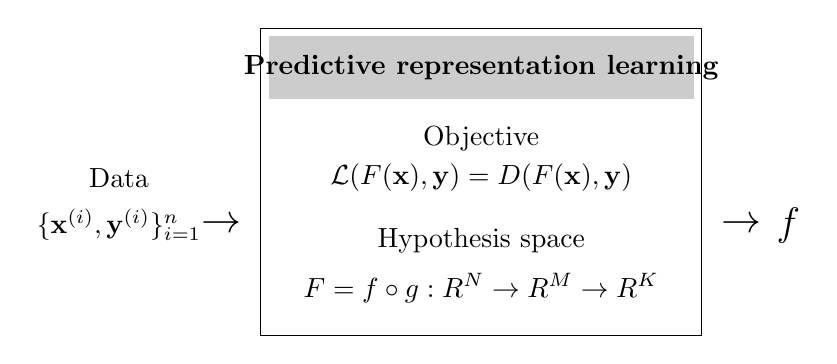
\begin{tikzpicture}
        \draw (0,0) rectangle (5.6,3.9); % outer box
        \fill[black!20] (0.1,3.0) rectangle (5.5,3.8); % gray box
        \node[] at (2.8,3.4) {{\bf Predictive representation learning}};
        \node[] at (2.8,2.5) {Objective}; \node[] at (2.8,2.0) {$\mathcal{L}(F(\mathbf{x}), \mathbf{y}) = D(F(\mathbf{x}), \mathbf{y})$};
            \node[] at (2.8,1.2) {Hypothesis space}; \node[] at (2.8,0.6) {$F = f \circ g: \mathbb{R}^N \rightarrow \mathbb{R}^M \rightarrow \mathbb{R}^K$};
            \node[] at (-1.8,2.0) {Data};
            \node[] at (-1.8,1.4) {$\{\mathbf{x}^{(i)}, \mathbf{y}^{(i)}\}_{i=1}^n$};
        \node[] at (-0.5,1.4) {{\Large  $ \rightarrow$}};
        \node[] at (6.7,1.4) {{\Large $f$}};
        \node[] at (6.1,1.4) {{\Large  $ \rightarrow$}};
    \end{tikzpicture}
\end{center}
where $D$ is some distance function, for example, $L_2$. Just like with the autoencoder, $f$ and $g$ are usually neural nets but may be any family of functions; often $g$ is just a single linear layer. Unlike with autoencoders, there is no standard setting for the relative dimensionalities of $N$, $M$, and $K$; instead it depends on the prediction task. If the task is image classification, then $N$ will be the (large) dimensionality of the input pixels, $M$ will usually be much lower dimensional, and $K$ will be the number of image classes (to output $K$-dimensional class probability vectors).

\subsection{Object Detectors Emerge from Scene-Level Supervision}
The real power of these pretexts tasks lies not in solving the tasks themselves but in acquiring useful image embeddings $\mathbf{z}$ as a byproduct of solving the pretext task. The amazing thing that ends up happening is that $z$-space may have \textit{emergent structure} that was not explicit in either the raw training data nor the pretext task. As a case study, consider the work of \cite{zhou2014object}. They trained a convolutional neural net (CNN) to perform scene classification, which asks whether the image shows a living room, bedroom, kitchen, and so on. The net did wonderfully at that task, but that wasn't the point. The researchers instead peeled apart the net and looked at which input images were causing different neurons within the net to fire. What they found was that there were neurons, on hidden layers in the net, that fired selectively whenever the input image was of a specific object class. For example, one particular neuron would fire when the input was a staircase, and another neuron would fire predominantly for inputs that were rafts. The subsequent images (\fig{\ref{fig:representation_learning:obj_detectors_emerge}}) show four of the top images that activate these two particular neurons. These particular neurons are on convolutional layers, so really each is a filter response; the highlighted regions indicate where the feature map for that filter exceeds a threshold.
\begin{figure}[h!]
    \centerline{
        \begin{minipage}{.3\linewidth}
            \begin{tikzpicture}
                %
                \def\Nlayers{3}
                \def\layerheight{0.8}
                \def\layerrad{0.4}
                \def\neuronrad{0.15}
                \def\neuronstep{0.7}
                \foreach \y in {1,...,\Nlayers} {
                        \draw (-\layerrad*\Nlayers+\layerrad*\y*0.5,\layerheight*\y) rectangle ++(\layerrad*\Nlayers*2-\layerrad*\y,\neuronrad*2);
                        \draw [nn_edge,thick] (0,\layerheight*\y+\neuronrad*2) -- (0,\layerheight*\y+\layerheight);
                    }
                \foreach \x in {1,...,4} {
                        \draw [fill=white] (\neuronrad*\x*2-5*\neuronrad,\layerheight*\Nlayers+\neuronrad) circle (\neuronrad);
                    }
                \draw (-\neuronrad,\layerheight*\Nlayers+\neuronrad) node {\scriptsize A};
                \draw (\neuronrad*2+\neuronrad,\layerheight*\Nlayers+\neuronrad) node {\scriptsize B};
                %
                \draw (0,\layerheight*\Nlayers+\layerrad+0.8) node {$\vdots$};
                \draw (0,\layerheight*\Nlayers+\layerrad+1.2) node {\texttt{scene label}};
                %\draw (\layerrad*\Nlayers-\layerrad*\y*0.5,\layerheight*\Nlayers+\neuronrad) node {$\Bigg\{$};
                \draw [dotted,thick] (\layerrad*\Nlayers-\layerrad*\Nlayers*0.5,\layerheight*\Nlayers+\neuronrad) -- (\layerrad*\Nlayers-\layerrad*\Nlayers*0.5+2.25,\layerheight*\Nlayers+\neuronrad+0.14);
                \draw [dotted,thick] (\layerrad*\Nlayers-\layerrad*\Nlayers*0.5,\layerheight*\Nlayers+\neuronrad) -- (\layerrad*\Nlayers-\layerrad*\Nlayers*0.5+2.25,\layerheight*\Nlayers+\neuronrad-1.1);
            \end{tikzpicture}
        \end{minipage}
        \begin{minipage}{.46\linewidth}
            \begin{tikzpicture}
                \draw (0, 0) node[inner sep=0] {\includegraphics[width=1.0\linewidth]{./figures/representation_learning/obj_detectors_emerge.pdf}};
                \draw (0,2) node {\small Images that maximally activate these neurons};
                % \vspace{0.7cm}
                % \begin{center}
                %     \includegraphics[width=1.0\linewidth]{figures/representation_learning/obj_detectors_emerge.pdf}
                % \end{center}
            \end{tikzpicture}
        \end{minipage}
    }
    \caption{Visualizing two neural receptive fields in a scene classifier neural net. Images taken from \cite{zhou2014object}.}
    \label{fig:representation_learning:obj_detectors_emerge}
\end{figure}

What this shows is that \textit{object} detectors, that is, neurons that selectively fire when they see a particular object class, emerge in the hidden layers of a CNN trained only to perform \textit{scene} classification. This makes sense in retrospect—how else would the net recognize scenes if not first by identifying their constituent objects?—but it was quite a shock for the community to see it for the first time. It gave some evidence that the way we humans parse and recognize scenes may match the way CNNs also internally parse and recognize scenes.

\section{Self-Supervised Learning}
\index{Self-supervised learning}
Predictive learning is great when we have good prediction targets that induce good representations. What if we don't have labeled targets provided to us? Instead we could try to cook up targets out of the raw data itself; for example, we could decide that the top right pixel's color will be the ``label'' of the image. This idea is called \textbf{self-supervision}. It looks like this:
\begin{center}
    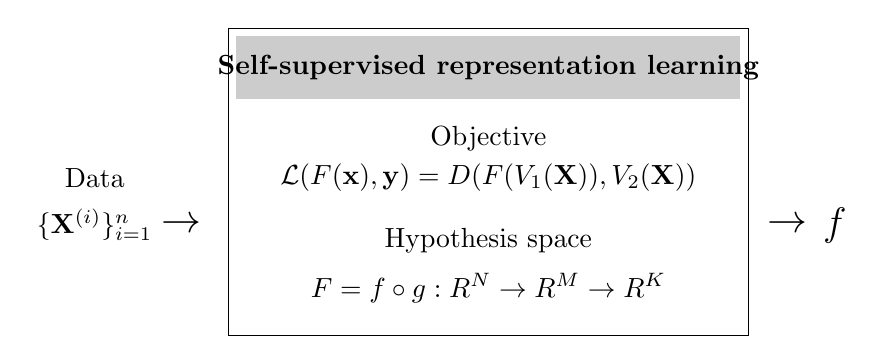
\begin{tikzpicture}
        \draw (0,0) rectangle (6.6,3.9); % outer box
        \fill[black!20] (0.1,3.0) rectangle (6.5,3.8); % gray box
        \node[] at (3.3,3.4) {{\bf Self-supervised representation learning}};
        \node[] at (3.3,2.5) {Objective}; \node[] at (3.3,2.0) {$\mathcal{L}(F(\mathbf{x}), \mathbf{y}) = D(F(V_1(\mathbf{X})), V_2(\mathbf{X}))$};
            \node[] at (3.3,1.2) {Hypothesis space}; \node[] at (3.3,0.6) {$F = f \circ g: \mathbb{R}^N \rightarrow \mathbb{R}^M \rightarrow \mathbb{R}^K$};
            \node[] at (-1.7,2.0) {Data};
            \node[] at (-1.7,1.4) {$\{\mathbf{X}^{(i)}\}_{i=1}^n$};
        \node[] at (-0.6,1.4) {{\Large  $ \rightarrow$}};
        \node[] at (7.7,1.4) {{\Large $f$}};
        \node[] at (7.1,1.4) {{\Large  $ \rightarrow$}};
    \end{tikzpicture}
\end{center}
where $V_1$ and $V_2$ are two different functions of the \textit{full data tensor} $\mathbf{X}$. For example, $V_1$ might be the left side of the image $\mathbf{X}$ and $V_2$ could be the right side, so the pretext task is to predict the right side of an image from its left side. In fact, several of the examples we gave previously for predictive learning are of the self-supervised variety: supervision for predicting a future frame, or a next pixel, can be cooked up just by splitting a video into past and future frames, or splitting an image into previous and next pixels in a raster-order sequence.

\section{Imputation}
\index{Imputation}{\bf Imputation} is a special case of self-supervised learning, where the prediction targets are missing elements of the input data. For example, predicting missing pixels is an imputation problem, as is colorizing a black and white photo (i.e., predicting missing color channels). \Fig{\ref{fig:representation_learning:imputation_examples}} gives several examples of these imputation tasks.
\begin{figure}[h!]
    \centerline{
        \includegraphics[width=1.0\linewidth]{figures/representation_learning/imputation_examples.pdf}
        \label{fig:representation_learning:imputation_examples}
    }
    \caption{Many common pretext tasks are special cases of imputation on missing values in the data tensor.}
    \label{fig:representation_learning:imputation_examples}
    \vspace{-1.0em}
\end{figure}

Imputation—whether over spatial masks or missing channels—can result in effective visual representations~\cite{vincent2008extracting, pathak2016context,he2022masked,zhang2016colorful,larsson2016learning,zhang2017split}. Notice that predicting future frames and next pixels (our examples from \fig{\ref{fig:representation_learning:predictive_learning_examples}}) are also imputation problems.

%[Example of how colorization can lead to semantic neurons]
%\paragraph{Object detectors emerge from colorization}
Above we described how object detectors emerge as a byproduct of training a net to perform scene classification. What do you think emerges as a byproduct of training a net to perform colorization?

It may surprise you to find that the answer is object detectors once again! This certainly surprised us when we saw the results in \fig{\ref{fig:representation_learning:obj_detectors_in_colorization}}, which are taken from \cite{zhang2016colorful}.
\begin{figure}[h!]
    \centerline{
        \begin{minipage}{.3\linewidth}
            \begin{tikzpicture}
                %
                \def\Nlayers{3}
                \def\layerheight{0.8}
                \def\layerrad{0.4}
                \def\neuronrad{0.15}
                \def\neuronstep{0.7}
                \foreach \y in {1,...,\Nlayers} {
                        \draw (-\layerrad*\Nlayers+\layerrad*\y*0.5,\layerheight*\y) rectangle ++(\layerrad*\Nlayers*2-\layerrad*\y,\neuronrad*2);
                        \draw [nn_edge,thick] (0,\layerheight*\y+\neuronrad*2) -- (0,\layerheight*\y+\layerheight);
                    }
                \foreach \x in {1,...,4} {
                        \draw [fill=white] (\neuronrad*\x*2-5*\neuronrad,\layerheight*\Nlayers+\neuronrad) circle (\neuronrad);
                    }
                \draw (-\neuronrad,\layerheight*\Nlayers+\neuronrad) node {\scriptsize A};
                \draw (\neuronrad*2+\neuronrad,\layerheight*\Nlayers+\neuronrad) node {\scriptsize B};
                %
                \draw (0,\layerheight*\Nlayers+\layerrad+0.8) node {$\vdots$};
                \draw (0,\layerheight*\Nlayers+\layerrad+1.6) node[inner sep=0] {\includegraphics[width=0.25\linewidth]{./figures/representation_learning/ab_bird.jpg}};
                %\draw (\layerrad*\Nlayers-\layerrad*\y*0.5,\layerheight*\Nlayers+\neuronrad) node {$\Bigg\{$};
                \draw [dotted,thick] (\layerrad*\Nlayers-\layerrad*\Nlayers*0.5,\layerheight*\Nlayers+\neuronrad) -- (\layerrad*\Nlayers-\layerrad*\Nlayers*0.5+2.25,\layerheight*\Nlayers+\neuronrad+0.4);
                \draw [dotted,thick] (\layerrad*\Nlayers-\layerrad*\Nlayers*0.5,\layerheight*\Nlayers+\neuronrad) -- (\layerrad*\Nlayers-\layerrad*\Nlayers*0.5+2.25,\layerheight*\Nlayers+\neuronrad-0.75);
            \end{tikzpicture}
        \end{minipage}
        \begin{minipage}{.5\linewidth}
            \begin{tikzpicture}
                \draw (0,0) node[inner sep=0] {\includegraphics[width=1.0\linewidth]{./figures/representation_learning/obj_detectors_in_colorization.pdf}};
                \draw (0,2) node {\small Images that maximally activate these neurons};
            \end{tikzpicture}
        \end{minipage}
    }
    \caption{Visualizing two neural receptive fields in the colorization model from \cite{zhang2016colorful}. Images generated by Andrew Owens and Richard Zhang.}
    \label{fig:representation_learning:obj_detectors_in_colorization}
\end{figure}

In fact, object detectors emerge in CNNs for just about any reasonable pretext task: scene recognition, colorization, inpainting missing pixels, and more. What may be going on is that these things we call ``objects'' are not just a peculiarity of human perception but rather map onto some fundamentally useful structure out there in the world, and any visual system tasked with understanding our world would arrive at a similar representation, carving up the sensory array into objects and other kinds of \textbf{perceptual groups}. This idea will be explored in greater detail in the next chapter. %roughly similar intelligence (e.g., an AI system, an alien on Mars) would learn to see the world in a similar way as we do.%, that is, as composed of the modular and compositional parts we call objects.

\section{Abstract Pretext Tasks}
Other varieties of self-supervised learning set up more abstract prediction problems, rather than just aiming to predict missing data. For example, we may try to predict if an image has been rotated 90 degrees~\cite{komodakis2018unsupervised}, or we may aim to predict the relative position of two image patches given their appearance~\cite{doersch2015unsupervised}. These pretext tasks can induce effective visual representations because solving them requires learning about semantic and geometric regularities in the world, such as that clouds tend to appear near the top of an image or that the trunk of a tree tends to appear below its branches.

\section{Clustering}
\index{Clustering}
One way to compress a signal is dimensionality reduction, which we saw an example of previously with the autoencoder. Another way is to quantize the signal into discrete categories, an operation known also as {\bf clustering}.\marginnote{Another name for clustering, more common in the representation learning literature, is \index{Vector quantization}\textbf{vector quantization}.} Mathematically, clustering is a function $f: \{\mathbf{x}^{(i)}\}_{i=1}^N \rightarrow \{1,\dots,k\}$, that is, a mapping from the members of a dataset $\{\mathbf{x}^{(i)}\}_{i=1}^N$ to $k$ integer classes ($k$ can potentially be unbounded). Representing integers with one-hot codes, clustering is shown in \fig{\ref{fig:representation_learning:clustering_f_diagram}}.
\begin{figure}[h!]
    \centerline{
        \includegraphics[width=0.4\linewidth]{figures/representation_learning/clustering_f_diagram.pdf}
    }
    \caption{You can think of clustering as being just like image labeling, except that that labels are self-discovered rather than being predefined.}
    \label{fig:representation_learning:clustering_f_diagram}
    \vspace{-1.0em}
\end{figure}


Clustering follows from the principle of compression: if we can well summarize a signal with just a discrete category label, then this summary can serve as a lighter weight and more abstracted substrate for further reasoning. You will already be familiar with clustering because we it in our natural language everyday. For example, consider the words ``antelope,'' ``giraffe,'' and ``zebra.'' Those words are discrete category labels (i.e., integers) that summarize huge conceptual sets (just think of all the individual lives and richly diverse personalities you are lumping together with the simple word ``antelope''). Words, then, are clusters! They are mappings from data to integers, and clustering is the problem of making up new words for things.\marginnote{Words, of course, are given additional structure when used in a language (grammar, connotations, etc.) beyond just being a set of clusters. The same kind of structure can be added on top of visual clusters.}

Many clustering algorithms not only partition the data but also compute a representation of the data within each cluster; this representation is sometimes called a \index{Code vector}\textbf{code vector}. The most common code vector is the \index{Clustering!Cluster center}\textbf{cluster center}, $\mu$, that is, the mean value of all datapoints assigned to the cluster. Clusters can also be represented by other statistics of the data assigned to them, such as the variance of this data or some arbitrary embedding vector, but this is less common. The set of cluster centers, $\{\mu_i\}_{i=1}^k$, is a representation of a whole data\textit{set}. They summarize the main modes of behavior in the dataset.

\subsection{$K$-Means}
\index{K-means}
There are many types of clustering algorithm but we will illustrate the basic principles with just one example, perhaps the most popular clustering algorithm of them all, $\mathbf{k}$\textbf{-means}. $K$-means is a clustering algorithm that partitions the data into $k$ clusters. Each datapoint $\mathbf{x}^{(i)}$ is assigned to a cluster indexed by an integer $a_i \in \{1, \ldots, k\}$. Each cluster is given a code vector $\mathbf{z} \in \mathbb{R}^M$. The $k$-means objective is to minimize the distance between each datapoint and the code vector of the cluster it is assigned to:
\begin{align}
    J_{\texttt{kmeans}} & = \sum_{i=1}^N \norm{\mathbf{z}_{a_i} - \mathbf{x}^{(i)}}^2_2 \quad\quad \triangleleft \quad\text{$k$-means objective}
\end{align}
This way, the code vector assigned to each datapoint will be a good approximation to the value of that datapoint, and we will have a faithful, but compressed, representation of the dataset.

There are two free parameter sets to optimize over: the code vectors and the cluster assignments. The cluster assignments can be represented with a clustering function $f: \{\mathbf{x}^{(i)}\}_{i=1}^N \rightarrow \{1,\dots,k\}$:
\begin{align}
    a_i = f(\mathbf{x}^{(i)})
\end{align}
We will represent the code vectors for each cluster with a function $g: \{1,\ldots,k\} \rightarrow \mathbb{R}^M$, where the data dimensionality is $M$:
\begin{align}
    \mathbf{z}_{a_i} = g(a_i)
\end{align}
Both $f$ and $g$ can be implemented as lookup tables, since for both the input is a countable set. The $k$-means algorithm amounts to just filling in these two lookup tables.

Now we are ready to present the full $k$-means algorithm, viewed as a learning algorithm. As you will see below, the learning diagram looks almost the same as for an autoencoder! The key differences are (1) the bottleneck is discrete integers rather than continuous vectors, and (2) the optimizer is slightly different (we will delve into it subsequently).%\marginnote{This chapter presents k-means as a representation learning algorithm and therefore forges a connection to another such algorithm we have seen: autoencoders. This is just one of many possible perspectives on k-means. Another way to motivate it is through a connection to Gaussian Mixture Models~\cite{XX}.}[-1cm]

%, and the clusters are represented by their centers, or ``means". The k-means objective is to minimize the distance between each datapoint and the mean of the cluster it is assigned to. This way, the mean assigned to each datapoint will be a good approximation to the value of that datapoint, and we will have a faithful, but compressed, representation of the dataset.
%The idea is that what the clustering tells us is just a mean 
%if we were to approximate each datapoint with the value of its cluster's mean, then we would not incur much error. In k-means, the error is measured by the distance (usually $L_2$) betweeen each datapoint and its assigned mean.
%The means are wiggled around to become closer to their assigned data and the cluster assignments are updated so that each datapoint is assigned to its closest mean.

%The objective of k-means is quite like an autoencoder, but one that compresses a data\textit{set} rather than compressing a data\textit{point}. The k-means objective,

%and we will present here one that follows a similar objective as the autoencoder. The {\bf k-means} algorithm is a bit like an autoencoder for a data\textit{set}, rather than a datapoint. It seeks to summarize a dataset with a set of $k$ clusters, such that if you only 

%seeks to summarize a dataset with a set of $k$ clusters. Each cluster will come with a ``mean" vector, $\mu$. The goal is to find the $\mu$'s that best summarize the datapoints assigned to each cluster.

%Each cluster may also come with some information that tells us about the datapoints assigned to that cluster. For example, a cluster might record the mean and/or variance of all the datapoints assigned to a cluster -- we will call these the cluster's features. In this way, each cluster is a \textit{summary} of the datapoints assigned to it, and clustering, therefore, follows from the compression principle: it summarizes a dataset with a set of \textit{cluster assignments for each datapoint} and a set of \textit{features for each cluster}. 

%There are many types of clustering algorithm and we will present here one that follows the same general objective as the autoencoder. 

%The {\bf k-means} objective aims to encode data into cluster assignments in such a way that the original data can be reconstructed as well as possible in an $L_2$ sense. Each cluster can be thought of as a summary of the datapoints assigned to that cluster, and in k-means the summary is represented just by the \textit{mean} of these datapoints. So, since we want to ``autoencode" the data as faithfully as possible, the k-means objective will be to assign each datapoint to the cluster whose mean is as close as possible to that datapoint. This way, if we were to just see the cluster assignments, we would know the rough values of the original datapoints. Mathematically, the objective is to assign each datapoint $\mathbf{x}$ to the cluster $j$ whose mean $\mu^{(j)}$ is closest to $\mathbf{x}$ in $L_2$ distance. The tricky bit of k-means is that the mean $\mu^{(j)}$ is a function of the cluster assignments.

%Below we formalize the k-means algorithm with a learning diagram. Here it helps to think of each cluster ``mean" not as the true mean of the datapoints assigned to that cluster, but instead as a free variable $\mu$ we will optimize over. It will turn out that the optimal value of $\mu$ is to set it to equal the true mean.
%learner as inferring both the clustering function $f$ and an auxiliary variable $\mathbf{U}$

\begin{center}
    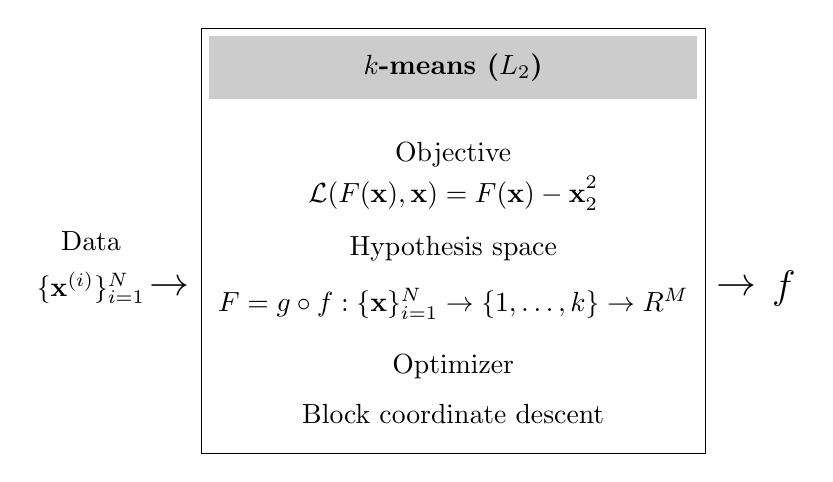
\begin{tikzpicture}
        \draw (0,0) rectangle (6.4,5.4); % outer box
        \fill[black!20] (0.1,4.5) rectangle (6.3,5.3); % gray box
        \node[] at (3.2,4.9) {{\bf $k$-means ($L_2$)}};
        %\node[] at (2.6,3.8) {Objective}; \node[] at (2.6,3.3) {$\sum_{j=1}^k 1(f(\mathbf{x}) = j) \left\Vert \mathbf{x} - \mathbf{\mu}^{(j)} \right\Vert_2^2$};
        %\node[] at (2.6,3.8) {Objective}; \node[] at (2.6,3.3) {$\mathcal{L}(\mathbf{x}; \mu, f) = \left\Vert \mathbf{x} - \mathbf{\mu}^{(f(\mathbf{x}))} \right\Vert_2^2$};
        %\node[] at (2.6,4.4) {Objective}; \node[] at (2.6,3.9) {$\mathcal{L}(\mathbf{x}; f, z) = \left\Vert \mathbf{x} - z(f(\mathbf{x})) \right\Vert_2^2$};
        \node[] at (3.2,3.8) {Objective}; \node[] at (3.2,3.3)
        {$\mathcal{L}(F(\mathbf{x}), \mathbf{x}) = \norm{F(\mathbf{x}) - \mathbf{x}}_2^2$};
            %\node[] at (2.6,3.1) {Hypothesis space}; \node[] at (2.6,2.5) {$f: \{\mathbf{x}\}_{i=1}^N \rightarrow \{1,\ldots,k\}$};
            %\node[] at (2.6,1.9) {$z: \{1,\ldots,k\} \rightarrow \mathbb{R}^M$};
            \node[] at (3.2,2.6) {Hypothesis space}; \node[] at (3.2,1.9) {$F = g \circ f: \{\mathbf{x}\}_{i=1}^N \rightarrow \{1,\ldots,k\} \rightarrow \mathbb{R}^M$};
            %\node[] at (2.6,2.5) {Hypothesis space}; \node[] at (2.6,1.9) {$f_{\mathbf{U}}(\mathbf{x}) = \argmin_j \left\Vert \mathbf{x} - \mathbf{\mu}^{(j)} \right\Vert^2_2 $};
            %\node[] at (2.6,2.5) {Hypothesis space}; \node[] at (2.6,1.9) {$f(\mathbf{x}^{(i)}) = \mathbf{j}^(i), \mu^{j} \in \mathbb{R}^N \forall j$};
            \node[] at (3.2,1.1) {Optimizer}; \node[] at (3.2,0.5) {Block coordinate descent};
            \node[] at (-1.4,2.7) {Data};
            \node[] at (-1.4,2.1) {$\{\mathbf{x}^{(i)}\}_{i=1}^N$};
        \node[] at (-0.4,2.1) {{\Large  $ \rightarrow$}};
        \node[] at (7.4,2.1) {{\Large $f$}};
        \node[] at (6.8,2.1) {{\Large  $ \rightarrow$}};
    \end{tikzpicture}
\end{center}

To recap, there are two functions we are optimizing over: the encoder $f$ and the decoder $g$. The $f$ is parameterized by a set of integers $\{a_i\}_{i=1}^N$,  $a_i \in \{1,\ldots,k\}$, which specify the cluster assignment for each datapoint. The decoder $g$ is parameterized by a set of $k$ code vectors $\{\mathbf{z}_j\}_{j=1}^k$, $\mathbf{z}_j \in \mathbb{R}^{M}$, one for each cluster, so we have $F(\mathbf{x}^{(i)}) = g(f(\mathbf{x}^{(i)})) = g(a_i) = \mathbf{z}_{a_i}$. The $g$ is differentiable with respect to its parameters but $f$ is not, because the parameters of $f$ are discrete variables. This means that gradient descent will not be a suitable optimization algorithm (the gradient $\frac{\partial f}{\partial a_i}$ is undefined). Instead, we will use the optimization strategy described next.

\subsubsection{Optimizing $k$-means} $K$-means uses an optimization algorithm called \index{Block coordinate descent}\textbf{block coordinate descent}. This algorithm splits up the optimization parameters into multiple subsets (blocks). Then it alternates between \textit{fully} minimizing the objective with respect to each block of parameters. In $k$-means there are two parameter blocks: $\{a_i\}_{i=1}^N$ and $\{\mathbf{z}_j\}_{j=1}^k$. So, we need to derive update rules that find the minimizer of the $k$-means objective with respect to each block. It turns out there are simple solutions for both:
\begin{align}
    %a_i &\leftarrow \argmin_j \norm{F(\mathbf{x}^{(i)}) - \mathbf{x}^{(i)}}_2^2\\
    a_i          & \leftarrow \argmin_{j \in \{1,\ldots,k\}} \norm{\mathbf{z}_j - \mathbf{x}^{(i)}}_2^2 \quad\quad \triangleleft\quad\text{Assign datapoint to nearest cluster}\label{eqn:representation_learning:kmeans_update_assignments} \\
    \mathbf{z}_j & \leftarrow \frac{1}{N}\sum_{i=1}^N \mathbbm{1}(a_i = j)\mathbf{x}^{(i)} \quad\quad \triangleleft\quad\text{Set code vector to cluster center}\label{eqn:representation_learning:kmeans_update_means}
\end{align}

These steps are repeated until a fixed point is reached, which occurs when all the datapoints that are assigned to each cluster are closest to that cluster's code vector.

Why are these the correct updates? \Eqn{\ref{eqn:representation_learning:kmeans_update_assignments}} is straightforward: it's just a brute force enumeration of all $k$ possible assignments, from which we select the one that minimizes the $k$-means objective for that datapoint, given the current set of code vectors $\{\mathbf{z}_j\}_{j=1}^k$.

\Eqn{\ref{eqn:representation_learning:kmeans_update_means}} is slightly trickier. It finds the optimal codes $\{\mathbf{z}_j\}_{j=1}^k$ given the current set of assignments $\{a_i\}_{i=1}^N$. To see why \eqn{\ref{eqn:representation_learning:kmeans_update_means}} is optimal, first rewrite the $k$-means objective as follows:
\begin{align}
    J_{\texttt{kmeans}} & = \sum_{i=1}^N \norm{\mathbf{z}_{a_i} - \mathbf{x}^{(i)}}^2_2                               \\
                        & = \sum_{j=1}^k \sum_{i=1}^N \mathbbm{1}(a_i = j) \norm{\mathbf{z}_j - \mathbf{x}^{(i)}}^2_2
\end{align}
%Our task is to minimize the objective over all datapoints, that is, $\sum_{i=1}^N \norm{\mathbf{z}_{a_i} - \mathbf{x}^{(i)}}^2_2$, which can be rewritten as $\sum_{j=1}^k \sum_{i=1}^N \mathbbm{1}(a_i = j) \norm{\mathbf{z}_j - \mathbf{x}^{(i)}}^2_2$. Each term in the outer sum is affected by only one of the $k$ $\mathbf{z}_j$. 
Looking at one code vector (the $j$-th) in isolation, we are seeking:
\begin{align}
    \argmin_{\mathbf{z}_j} \sum_{i^{\prime} \text{ s.t. } a_{i^\prime}=j} \norm{\mathbf{z}_j - \mathbf{x}^{(i^{\prime})}}^2_2
\end{align}
where $i^{\prime}$ enumerates all the datapoints for which $a_{i^\prime} = j$. Recall that the point that minimizes the sum of squared distances from a dataset is the mean of the dataset. This yields our update in \eqn{\ref{eqn:representation_learning:kmeans_update_means}}: just set each code to be the mean of all datapoints assigned to that code's cluster.

Now we can see where the name $k$-means comes from: the optimal code vectors are the cluster \textit{means}. The algorithm is very simple: compute the cluster means given current data assignments; reassign each datapoint to nearest cluster mean; recompute the means; and so on until convergence. An example of applying this algorithm to a simple dataset of two-dimensional (2D) points is given in \fig{\ref{fig:representation_learning:kmeans_ex}}.

\begin{figure}[t]
    \centerline{
        \begin{subfigure}{0.25\textwidth}
            \includegraphics[width=\linewidth]{figures/representation_learning/kmeans_ex_step1.jpg}
            \caption*{(a)}
        \end{subfigure}%
        \hspace*{\fill}   % maximize separation between the subfigure
        \begin{subfigure}{0.25\textwidth}
            \includegraphics[width=\linewidth]{figures/representation_learning/kmeans_ex_step2.jpg}
            \caption*{(b)}
        \end{subfigure}%
        \hspace*{\fill}   % maximize separation between the subfigure
        \begin{subfigure}{0.25\textwidth}
            \includegraphics[width=\linewidth]{figures/representation_learning/kmeans_ex_step3.jpg}
            \caption*{(c)}
        \end{subfigure}%
        \hspace*{\fill}   % maximize separation between the subfigure
        \begin{subfigure}{0.25\textwidth}
            \includegraphics[width=\linewidth]{figures/representation_learning/kmeans_ex_step4.jpg}
            \caption*{(d)}
        \end{subfigure}%
    }
    \caption{Iterations of $k$-means applied to a simple 2D dataset, with $k=5$. The code vectors assigned to each cluster are marked with an x. (a) Initialization. (b) Update code vector to be cluster means. (c) Update assignments. (d) Converged solution (which occurs here after four updates of both codes and assignments)}
    \label{fig:representation_learning:kmeans_ex}
\end{figure}

\subsection{$K$-Means from Multiple Perspectives}
This section has presented $k$-means as a representation learning algorithm. In other texts you may encounter other views on $k$-means, for example, as a way of interpreting your data or as a simple generative model. These views are all complementary and all simultaneously true. Here we showed that $k$-means is like an autoencoder with a discrete bottleneck. In the next chapters we will encounter generative models, including one called a Gaussian mixture model (GMM). $K$-means can also be viewed as a vanilla form of a GMM. Later we will show that another kind of autoencoder, called a variational autoencoder (VAE), is a continuous version of a GMM. So we have a rich tapestry of relationships: autoencoders and VAEs are continous versions of $k$-means and GMMs, respectively. GMMs and VAEs are formal probabilistic models that, respectively, extend $k$-means and autoencoders (which do not come with probabilistic semantics). This is just one set of connections that can be made. In this book, be on the lookout for more connections like this. It can be confusing at first to see multiple different perspectives on the same method: Which one is correct? But rarely is there a single correct perspective. It is useful to identify the delta between each new model you encounter and all the models you already know. Usually there is a small delta with respect to \textit{many} things you already know, and rarely is there no meaningful connection between any two arbitrary models. As an exercise, try picking a random concept on a random page in this book (or, for a challenge, any book on your bookshelf). What is the delta between that concept and $k$-means, or between that concept and a different concept on any other random page? In our experience, it will often be surprisingly small (but sometimes it takes a lot of effort to see the connection).

%The parameters being learned are a set of cluster centers $\mathbf{U} \triangleq \{\mathbf{\mu}\}_{i=1}^k$. To optimize we could use standard gradient descent, but for k-means we typically use a slightly different descent algorithm, \textbf{block coordinate descent}, which can have faster convergence. The way this works is to 

%One other difference is that the ``encoder" $f$ is just a lookup table and therefore cannot encode arbitrary new datapoints that were not in the training set. However, we can easily 

%We could certainly use regular gradient descent, but a small trick makes convergence faster: it turns out that 

%Gradient descent on the k-means objective, w.r.t. cluster centers, ends up having a very simple form: on each step, each cluster center is simply updated to have the value of the mean of the datapoints that are ``assigned to" that cluster, i.e. for cluster $j$ this is those datapoints $\mathbf{x}$ such that $f_{\mathbf{U}}(\mathbf{x}) = j$.
%Block coordinate descent is the typical optimization algorithm for k-means. It is the same as gradient descent except that descent alternates between assigning datapoints to the nearest cluster center and updating the cluster center to be the mean of the assigned datapoints (each of these operations is a gradient step on the objective, just with respect to  different subset of the optimization variables).

\subsection{Clustering in Vision} In vision, the problem of clustering is related to the idea of \index{Perceptual grouping}\textbf{perceptual grouping}, which we cover in detail in \chap{\ref{chapter:perceptual_organization}}. We humans see the world as organized into different levels of perceptual structure: contours and surfaces, objects and events. These structures are groupings, or clusters, of related visual elements: a contour is a group of points that form a line, an object is a group of parts that form a cohesive, nameable whole, and so on. Algorithms like $k$-means, in a suitable feature space, can discover them.


\section{Contrastive Learning}\label{sec:representation_learning:contrastive_learning}
\index{Contrastive learning}

Dimensionality reduction and clustering algorithms learn compressed representations by creating an \index{Information bottleneck}{\bf information bottleneck}, that is, by constraining the number of bits available in the representation. An alternative compression strategy is to \textit{supervise} what information should be thrown away. {\bf Contrastive learning} is one such approach where a representation is supervised to be \textit{invariant} to certain viewing transformations, resulting in a compressed representation that only captures the properties that are common between the different data \textbf{views}. Two different data views could correspond to two different cameras looking at the same scene or two different imaging modalities, such as color and depth, and we will see more examples subsequently.\marginnote{Contrastive learning is actually more closely related to clustering than it may at first seem. Contrastive learning maps similar datapoints to similar embeddings. Clustering is just the extreme version of this where there are only $k$ distinct embeddings and similar datapoints get mapped to the \textit{exact same} embedding.}[-0.4cm]

Learning invariant representations is classic goal of computer vision. Recall that this was one of the reasons we used convolutional image filters: convolution is equivariant with camera translation, and invariance can then be achieved simply by pooling over filter responses. CNNs, through their convolutional architecture, bake translation invariance into the \textit{hypothesis space}. In this section we will see how to incentivize invariances instead through the \textit{objective} function.

The idea is to simply penalize deviations from the invariance we want. Suppose $T$ is a transformation we wish our representation to be invariant to. Then we may use a loss of the form $\norm{f(T(\mathbf{x}))-f(\mathbf{x})}_2^2$ to learn an encoder $f$ that is invariant to $T$. We call such a loss an \textbf{alignment} loss~\cite{wang2020hypersphere}.

That seems easy enough, but you may have noticed a flaw: What if $f$ just learns to output the zero vector all the time? Trivial alignment can be achieved when there is representational collapse, and all datapoints get mapped to the same arbitrary vector.

Contrastive learning fixes this issue by coupling an alignment loss with a second loss that pushes apart embeddings of datapoints for which we do not want an invariant representation. The supervision for contrastive learning comes in the form of \textit{positive pairs} and \textit{negative pairs}. Positive pairs are two datapoints we wish to align in $z$-space; if we wish for invariance to $T$ then a positive pair should be constructed as $\{\mathbf{x}, \mathbf{x}^{+}\}$ with $\mathbf{x}^{+} = T(\mathbf{x})$. Negative pairs, $\{\mathbf{x},\mathbf{x}^-\}$, are two datapoints that should be represented differently in $z$-space. Commonly, negative pairs are randomly constructed by sampling two datapoints independently and identically from the same data distribution, that is, $\mathbf{x} \sim p_{\texttt{data}}(\mathbf{x})$ and $\mathbf{x}^{-} \sim p_{\texttt{data}}(\mathbf{x})$. Given such data pairings, the objective is to pull together the positive pairs and push apart the negative pairs, as illustrated in \fig{\ref{fig:representation_learning:contrastive_learning_diagram}}.
\begin{figure}[h!]
    \centerline{
        \includegraphics[width=0.75\linewidth]{figures/representation_learning/contrastive_learning_diagram.pdf}
    }
    \caption{Contrastive learning.}
    \label{fig:representation_learning:contrastive_learning_diagram}
\end{figure}

This kind of contrastive learning results in an embedding that is invariant to a transformation $T$. Extending this to achieve invariance to a \textit{set} of transformations $\{T_1, \ldots, T_n\}$ is straightforward: just apply the same loss for each of $T_1, \ldots, T_n$.

A second kind of contrastive learning is based on co-occurrence, where the goal is to learn a common representation of all co-occurring signals. This form of contrastive learning is useful for learning, for example, an audiovisual representation where the embedding of an image matches the embedding of the sound for that same scene. Or, returning to our colorization example, we can learn an image representation where the embedding of the grayscale channels matches the embedding of the color channels. In both these cases we are learning to align co-occurring sensory signals. This kind of contrastive learning is schematized in \fig{\ref{fig:representation_learning:contrastive_learning_colorization}}.
\begin{figure}[h!]
    \centerline{
        \includegraphics[width=0.53\linewidth]{figures/representation_learning/contrastive_learning_colorization.pdf}
    }
    \caption{Contrastive learning from multiple views of the data. Figure inspired by \cite{tian2020contrastive}.}
    \label{fig:representation_learning:contrastive_learning_colorization}
\end{figure}

In \fig{\ref{fig:representation_learning:contrastive_learning_colorization}}, we refer to the two co-occurring signals—color and grayscale—as two different \index{Views (representation learning)}\textbf{views} of the total data tensor $\mathbf{X}$, just like we did in the previous sections: $\mathbf{x} = V_1(\mathbf{X})$, $\mathbf{y} = V_1(\mathbf{X})$. You can think of these views either as resulting from sensory co-occurrences or as two transformations of $\mathbf{X}$, where the transformation in the color example is channel dropping. Thus, the two kinds of contrastive learning we have presented are really one and the same: any two signals can be considered transformations of a combined total signal, and any signal and its transformation can be considered two co-occurring ways of measuring the underlying world.

Nonetheless, it is often easiest to conceptualize these two approaches separately, and next we give learning diagrams for each:
%The first is contrastive learning to learn an embedding invariant to a transformation $T$. Extending this to achieve invariance to a \textit{set} of transformations $\{T_1, \ldots, T_n\}$ is straightforward. The second is contrastive learning based on co-occurrence, where the goal is to learn a common representation of all co-occurring signals. This form of contrastive learning is useful for learning, e.g., an audiovisual representation where the embedding of an image matches the embedding of the sound for that same scene.
\begin{center}
    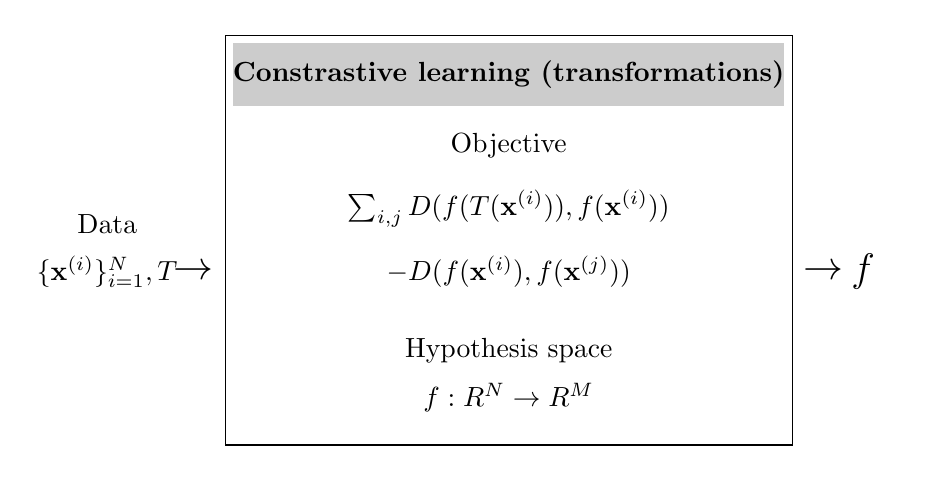
\begin{tikzpicture}
        \draw (0,0) rectangle (7.2,5.2); % outer box
        \fill[black!20] (0.1,4.3) rectangle (7.1,5.1); % gray box
        \node[] at (3.6,4.7) {{\bf Constrastive learning (transformations)}};
        \node[] at (3.6,3.8) {Objective}; \node[] at (3.6,3.0) {$\sum_{i,j} D(f(T(\mathbf{x}^{(i)})), f(\mathbf{x}^{(i)}))$}; \node[] at (3.6,2.2) {$- D(f(\mathbf{x}^{(i)}), f(\mathbf{x}^{(j)}))$};
        \node[] at (3.6,1.2) {Hypothesis space}; \node[] at (3.6,0.6) {$f: \mathbb{R}^N \rightarrow \mathbb{R}^M$};
        \node[] at (-1.5,2.8) {Data};
        \node[] at (-1.5,2.2) {$\{\mathbf{x}^{(i)}\}_{i=1}^N, T$};
        \node[] at (-0.4,2.2) {{\Large  $ \rightarrow$}};
        \node[] at (8.1,2.2) {{\Large $f$}};
        \node[] at (7.6,2.2) {{\Large  $ \rightarrow$}};
        %
        \useasboundingbox (-2,-0.1) rectangle (8.75,5.3);
    \end{tikzpicture}
\end{center}

\begin{center}
    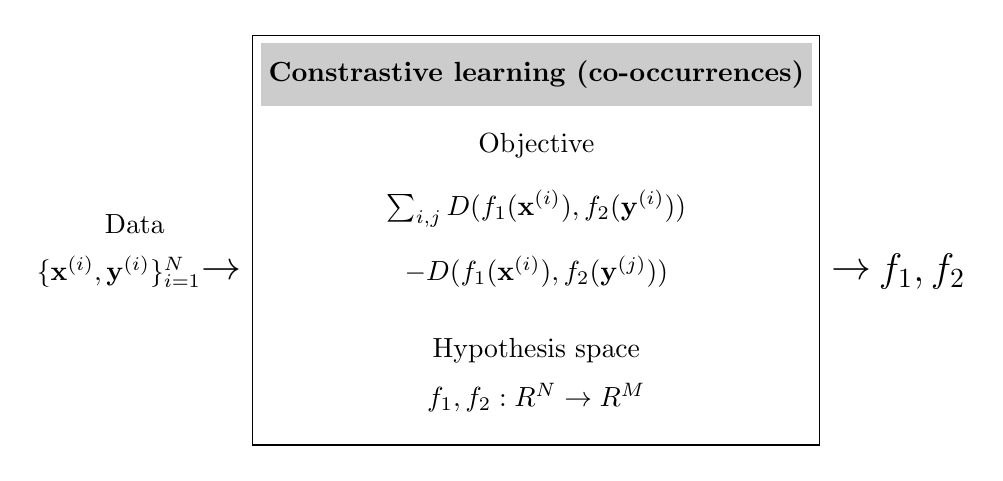
\begin{tikzpicture}
        \draw (0,0) rectangle (7.2,5.2); % outer box
        \fill[black!20] (0.1,4.3) rectangle (7.1,5.1); % gray box
        \node[] at (3.6,4.7) {{\bf Constrastive learning (co-occurrences)}};
        \node[] at (3.6,3.8) {Objective}; \node[] at (3.6,3.0) {$\sum_{i,j} D(f_1(\mathbf{x}^{(i)}), f_2(\mathbf{y}^{(i)}))$}; \node[] at (3.6,2.2) {$- D(f_1(\mathbf{x}^{(i)}), f_2(\mathbf{y}^{(j)}))$};
        \node[] at (3.6,1.2) {Hypothesis space}; \node[] at (3.6,0.6) {$f_1, f_2: \mathbb{R}^N \rightarrow \mathbb{R}^M$};
        \node[] at (-1.5,2.8) {Data};
        \node[] at (-1.7,2.2) {$\{\mathbf{x}^{(i)}, \mathbf{y}^{(i)}\}_{i=1}^N$};
        \node[] at (-0.4,2.2) {{\Large  $ \rightarrow$}};
        \node[] at (8.5,2.2) {{\Large $f_1, f_2$}};
        \node[] at (7.6,2.2) {{\Large  $ \rightarrow$}};
        %
        \useasboundingbox (-2,-0.1) rectangle (9,5.3);
    \end{tikzpicture}
\end{center}

In these diagrams, $D$ is a distance function. Above we give just one simple form for the contrastive objective; many variations have been proposed. Three of the most popular are (1) Hadsell et al.'s \index{Contrastive learning!Contrastive loss}``constrastive loss'' \cite{hadsell2006dimensionality} (an older definition of the term, now overloaded with our more general notion of a contrastive loss being the broader family of any loss that pulls together positive samples and pushes apart negative samples), (2) the \index{Contrastive learning!Triplet loss}\textbf{triplet loss} \cite{chechik2010large}, and (3) the \index{Contrastive learning!InfoNCE loss}\textbf{InfoNCE loss} \cite{oord2018representation}. Hadsell et al.'s contrastive loss and the triplet loss add the concept of a \index{Margin}\textbf{margin} to the vanilla formulation: they only push/pull when the distance is less than a specified amount $m$ (called the margin), otherwise points are considered far enough apart (or close enough together). The InfoNCE loss is a variation that treats establishing a contrast as a classification problem: it tries to move points apart until you can classify the positive sample, for a given anchor, separately from all the negatives. The general formulation of these losses takes as input an anchor $\mathbf{x}$, a positive example $\mathbf{x}^+$, and one or more negative examples $\mathbf{x}^-$. The positive and negative may be defined based on transformations, coocurrences, or something else. The full learning objective is to sum over many samples of anchors, positives, and negatives, producing a sampled set evaluated according to the losses as follows:
%\marginnote{``Contrastive loss" is an overloaded terms. Historically it referred to a specific loss from metric learning; in this book, following current practice, we will use it to refer to any loss function that pulls together positive pairs and pushes apart negative pairs.}
\begin{align}
    \mathcal{L}(\mathbf{x}, \mathbf{x}^+, \mathbf{x}^-)               & = \max(D(f(\mathbf{x}), f(\mathbf{x}^+)-m_{\texttt{pos}},0) - \nonumber                                                                                                                                                                                                                       \\ &\quad \max(m_{\texttt{neg}} - D(f(\mathbf{x}), f(\mathbf{x}^-),0) \quad \triangleleft \quad \text{Hadsell et al. ``contrastive''}\\
    \mathcal{L}(\mathbf{x}, \mathbf{x}^+, \mathbf{x}^-)               & = \max(D(f(\mathbf{x}), f(\mathbf{x}^+)) - D(f(\mathbf{x}), f(\mathbf{x}^-)) + m, 0) \quad\quad \triangleleft \quad \text{triplet}                                                                                                                                                            \\
    \mathcal{L}(\mathbf{x}, \mathbf{x}^+, \{\mathbf{x}_i^-\}_{i=1}^N) & = -\log \frac{e^{f(\mathbf{x})^\transpose f(\mathbf{x}^+)/\tau}}{e^{f(\mathbf{x})^\transpose f(\mathbf{x}^+)/\tau} + \sum_i e^{f(\mathbf{x})^\transpose f(\mathbf{x}_i^-)/\tau}} \quad\quad\quad\quad\quad\quad\triangleleft \quad \text{InfoNCE} \label{eqn:representation_learning:infonce}
\end{align}
\marginnote{Here $m$ is a general margin parameter, and $m_{\texttt{pos}}$ and $m_{\texttt{neg}}$ are separate margins for the positive and negative pairs respectively.}[-4.0cm]
Notice that the InfoNCE loss is a log softmax over a vector of scores $f_1(\mathbf{x})^\transpose f_2(c)/\tau$ with $c \in \{\mathbf{x}^+, \mathbf{x}_1^-, \ldots, \mathbf{x}_N^-\}$; you can therefore think of this loss as corresponding to a classification problem where the ground truth class is $\mathbf{x}^+$ and the other possible classes are $\{\mathbf{x}_1^-, \ldots, \mathbf{x}_N^-\}$ (refer to \chap{\ref{chapter:intro_to_learning}} to revisit softmax classification).

\subsection{Alignment and Uniformity}
\index{Contrastive learning!Alignment and uniformity}
Wang and Isola~\cite{wang2020hypersphere} showed that the contrastive loss (specifically the InfoNCE form) encourages two simple properties of the embeddings: alignment and uniformity. We have already seen that alignment is the property that two views in a positive pair will map to the same point in embedding point, that is, the mapping is invariant to the difference between the views. \textbf{Uniformity} comes from the negative term, which encourages embeddings to spread out and tend toward an evenly spread, uniform distribution. Importantly, for this to work out mathematically, the embeddings must be \textit{normalized}, that is, each embedding vector must be a unit vector. Otherwise, the negative term can push embeddings toward being infinitely far apart from each other. Fortunately, it is standard practice in contrastive learning (and many other forms of representation learning) to apply $L_2$ normalization to the embeddings. The result is that the embeddings will tend toward a uniform distribution over the surface of the $M$-dimensional hypersphere, where $M$ is the dimensionality of the embeddings. See theorem 1 in \cite{wang2020hypersphere} for a formal statement of this fact.

A result of this analysis is we may explicit decompose contrastive learning into one loss for alignment and another for uniformity, with the following forms:
\begin{align}
    \mathcal{L}_{\texttt{align}}(f;\alpha) & = \mathbb{E}_{(\mathbf{x},\mathbf{x}^+) \sim p_{\texttt{pos}}} [\norm{f(\mathbf{x}) - f(\mathbf{x}^+)}_2^{\alpha}]                               \\
    \mathcal{L}_{\texttt{unif}}(f;t)       & = \log \mathbb{E}_{\mathbf{x} \sim p_{\texttt{data}}, \, \mathbf{x}^- \sim p_{\texttt{data}}} [e^{-t\norm{f(\mathbf{x}) - f(\mathbf{x}^-)}_2^2}] \\
    \mathcal{L}(f;\alpha,t,\lambda)        & = \mathcal{L}_{\texttt{align}}(f;\alpha) + \lambda \mathcal{L}_{\texttt{unif}}
\end{align}
where $p_{\texttt{pos}}$ is the distribution of positive pairs and $\alpha$, $t$, and $\lambda$ are hyperparameters of the losses.

\subsection{Experiment: Designing Embeddings with Contrastive Learning}\label{sec:representation_learning:expt_designing_embeddings_with_contrastive_learning}
Using the alignment and uniformity objective defined previously, we will now illustrate how one can design embeddings with desired invariances. We will use the shape dataset described in \sect{\ref{sec:representation_learning:autoencoders}}, and will use the same encoder architecture and optimizer as from that section (a CNN with six layers, Adam optimizer, 20,000 iterations of stochastic gradient descent, batch size of 128). In contrast to the autoencoder experiment, however, we will set the dimensionality of the embedding to $M=2$, so that we can visualize it in a 2D plot.

\begin{figure}[t!]
    \centerline{
        \includegraphics[width=1.0\linewidth]{figures/representation_learning/align_unif_results_shapes_dataset.pdf}}
    \caption{Contrastive learning on colored shapes using two different transformations for creating positive pairs. The choice of transformation controls which features the embedding becomes sensitive to and which it becomes invariant to.}
    \label{fig:representation_learning:align_unif_results_shapes_dataset}

\end{figure}

Suppose we wish to obtain an embedding that is sensitive to color and invariant to shape. Then we should choose a view transformation $T_{\texttt{c}}$ that preserves color while changing shape. A simple choice that turns out to work is for $T_{\texttt{c}}(\mathbf{x})$ to simply output a crop from the image $\mathbf{x}$ (this transformation does not really change the object's shape but still ends up resulting in shape-invariant embeddings because color is a much more obvious cue for the CNN to pick up on and use for solving the contrastive problem). The result of contrastive learning, using $L_{\texttt{align}} + L_{\texttt{unif}}$ on data generated from $T_{\texttt{c}}$ is shown on the top row of \fig{\ref{fig:representation_learning:align_unif_results_shapes_dataset}}. Notice that the trained $f$ maps colors to be clustered into the color classes of this toy data, and that these classes become spread out more or less uniformly across the surface of a circle in embedding space (a one-dimensional hypersphere, because the embeddings are 2D and normalized).

We can repeat the same experiment but with a view transformation $T_{\texttt{s}}$ designed to be invariant to color. To do so we simply use the same transformation as for $T_{\texttt{c}}$ (i.e., cropping) plus add a random shift in hue, brightness, and saturation. Training on views generated from $T_{\texttt{s}}$ results in the embeddings on the bottom row of \fig{\ref{fig:representation_learning:align_unif_results_shapes_dataset}}. Now the embeddings become invariant to color but cluster shapes and spread out the three shape types to be roughly uniformly spaced around the hypersphere.


\section{Concluding Remarks}

This chapter, like much of this book, is about representations. Different representations make different problems easy, or hard. It is important to remember that every representation involves a set of tradeoffs: a good representation for one task may be a bad representation for another task. One of the current goals of computer vision research is to find \textit{general-purpose representations}, and what this means is not that the representation will be good for all tasks but that it will be good for a wide variety of the tasks that humans care about, which is a very tiny subset of all possible tasks.

% Classical vision hierarchy

% Representations in the brain

% Learning via compression
% Autoencoders

% Learning via prediction
% Self-supervised learning

% Invariance and equivariance

% Learning via generative modeling

% Clustering

% The view from information theory

% The view from metric learning


%\Section{Embeddings}